\documentclass[../main.tex]{subfiles}
\graphicspath{{img},{img/ink},{ink}}

\begin{document}

\begin{tcolorbox}[
    width=\textwidth,
    height=\textheight,
    title=Phyphox: Fallschnur,
    fonttitle=\Large,
    before title=\vspace{0.2cm}, after title=\vspace{0.2cm},
    colback=white,
    title filled=true, 
    colbacktitle=myorange,
    colframe=black,
    coltitle=black,
    ]

    \begin{minipage}[]{0.75\textwidth}

        \begin{minipage}[]{0.75\textwidth}
            \textbf{Klassenstufe}: 9/10

            \vspace{0.5cm}

            \textbf{Fachlicher Bezug}: Freier Fall, Erdbeschleunigung

            \vspace{0.5cm}
            \textbf{Material}: 
            \begin{itemize}[noitemsep]
                \item Schnur ca. $2\,$ m
                \item 6-7 Schrauben + Muttern
                \item Backblech
                \item 2 Handys + Phyphox 
            \end{itemize}

        \end{minipage}
        \hspace{0.2cm}
        \begin{minipage}[]{0.20\textwidth}
            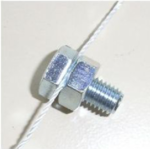
\includegraphics[width=1\textwidth]{img/schraube}

            \vspace{0.1cm}
            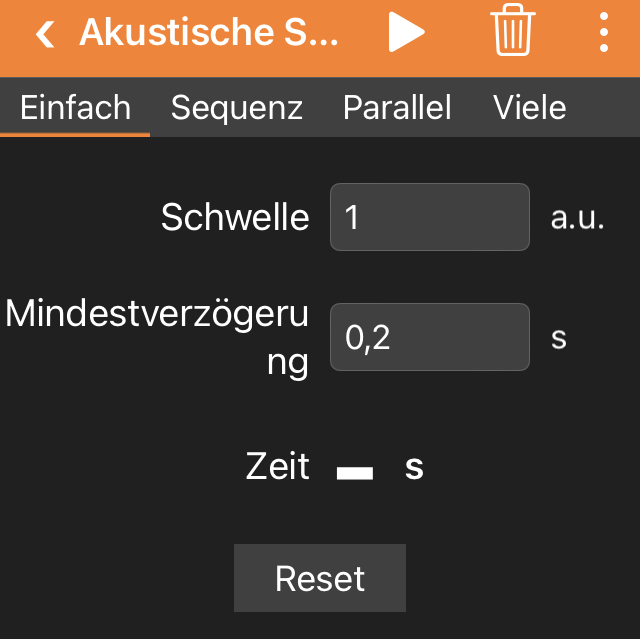
\includegraphics[width=1\textwidth]{img/app1}
        \end{minipage}

        \vspace{0.5cm}
        \textbf{Aufbau}: An einer Schnur werden Schrauben mit Muttern angebracht. Dabei wird ein Verhältnis von ungeraden Zahlen $1:3:5:7:\ldots$ verwendet. Auf einem Handy wird die Phyphox-App gestartet. Im Reiter \glqq Zeitmessung\grqq{} wird die \glqq Akustische Stoppuhr \grqq{} ausgewählt. Im Tab \glqq Einfach\grqq{} wird die Schwelle $=1$ und die Mindesverzögerung $=0,1$ gesetzt (ggf. selber anpassen). Der Fernzugriff wird aktiviert und das Handy wird unter dem Backblech platziert. Das zweite Handy wird über den Fernzugriff mit dem Experiment verbunden und die \glqq Sequenz\grqq{}-Messung ausgewählt.
    \end{minipage}
    \hspace{0.5cm}
    \begin{minipage}[]{0.2\textwidth}
        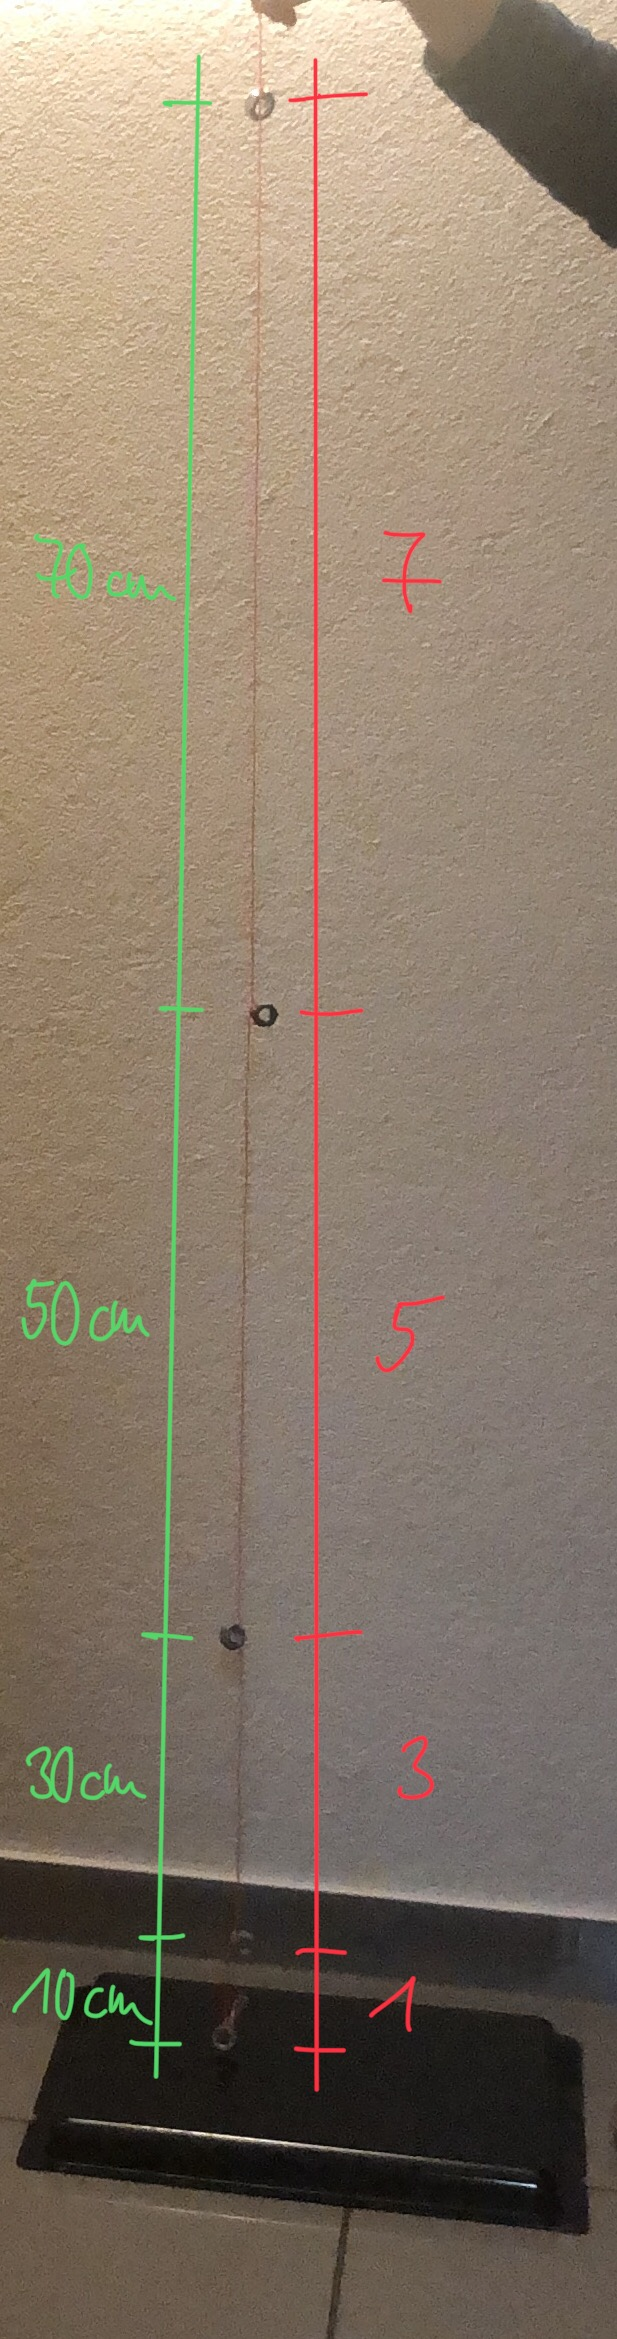
\includegraphics[width=0.85\textwidth]{img/versuchsaufbau}
    \end{minipage}

    \vspace{-0.8cm}

    \begin{minipage}[]{0.7\textwidth}
        \textbf{Durchführung}:   Die Schnur wird am oberen Ende gehalten, sodass die erste Schraube (dieser Aufschlag startet die Messung) mit etwas Abstand über dem Backblech hängt. Das Experiment wird gestartet und die Schnur losgelassen.

        \vspace{0.5cm}
        \textbf{Ergebnis}: Man beobachtet ein regelmäßiges Aufschlagen der Schrauben. Auch in der Phyphox-App misst man dieselben Zeiten zwischen dem Auftreffen der einzelnen Schrauben. Daraus folgt die Proportionalität
        \begin{align*}
            s \sim t^2
        \end{align*}
        Kennen die SuS die Formel für Bewegungen mit konstanter Beschleunigung $a$
        \begin{align*}
            s(t) = \frac{1}{2} \cdot a \cdot  t^2
        \end{align*}
        folgt, dass auch die Erdbeschleunigung $g$ einen festen Wert besitzen muss.\\
        Die Zusammenhänge lassen sich über einer dimensionslosen Betrachtung in Tabellenform verdeutlichen (dabei gilt $\Delta t \, \widehat{=} \, 1$ $\Rightarrow$ $\Delta s \,\widehat{=}\, v$ und $\Delta(\Delta s)\,\widehat{=}a$).
    \end{minipage}
    \hspace{0.2cm}
    \begin{minipage}[]{0.2\textwidth}
        \vspace{1.3cm} 
        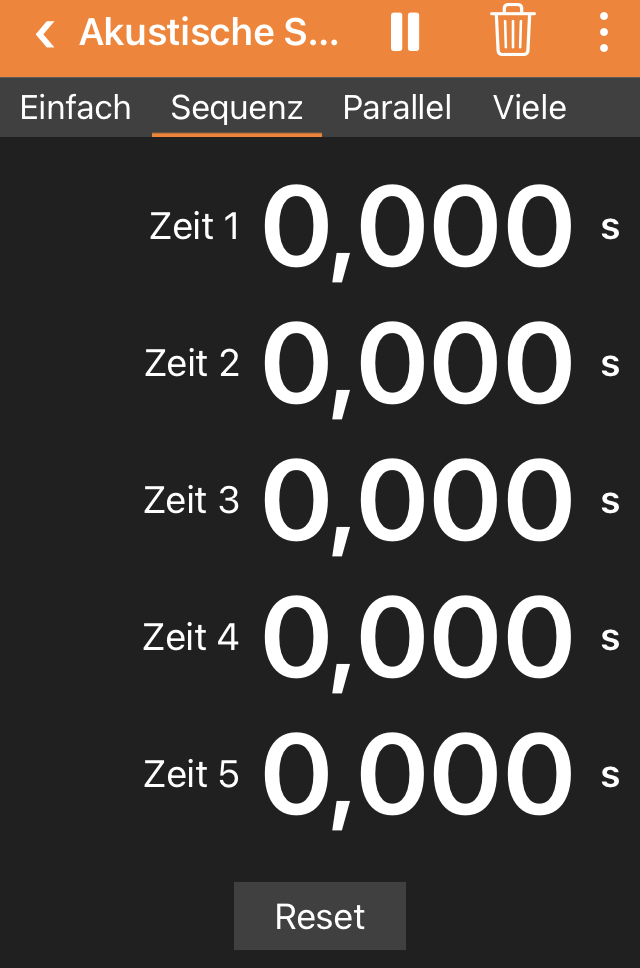
\includegraphics[width=1.2\textwidth]{img/app2}
        
        \vspace{-0.2cm}
        \begin{table}[H]
            \centering
            \begin{tabularx}{\textwidth}{ c c c c }
                \rowcolor{tablegray1} 
                t & s & $\Delta s$ & $\Delta(\Delta s)$ \\ \cline{1-4}
                \rowcolor{tablegray2}
                0 & 0 \tikzmark{brace0} &  & \\
                  & & 1 \tikzmark{brace5} & \\
                  \rowcolor{tablegray2}
                1 & 1 \tikzmark{brace1} &  & 2\\
                  & & 3 \tikzmark{brace6} & \\
                  \rowcolor{tablegray2}
                2 & 4 \tikzmark{brace2} &  & 2\\
                  & & 5 \tikzmark{brace7} & \\
                  \rowcolor{tablegray2}
                3 & 9 \tikzmark{brace3} &  & 2\\
                  & & 7 \tikzmark{brace8} & \\
                  \rowcolor{tablegray2}
                4 & 16 \tikzmark{brace4} &  &
            \end{tabularx} 
        \end{table}

        \begin{tikzpicture}[remember picture,overlay]
            % Simple brace
            \draw [decorate,
                decoration = {brace}] ( [xshift=0.2cm, yshift=0.1cm] pic cs:brace0) -- ( [xshift=0.2cm, yshift=0.12cm] pic cs:brace1);
            \draw [decorate,
                decoration = {brace}] ( [xshift=0.2cm, yshift=0.08cm] pic cs:brace1) -- ( [xshift=0.2cm, yshift=0.12cm] pic cs:brace2);
            \draw [decorate,
                decoration = {brace}] ( [xshift=0.2cm, yshift=0.08cm] pic cs:brace2) -- ( [xshift=0.2cm, yshift=0.12cm] pic cs:brace3);
            \draw [decorate,
                decoration = {brace}] ( [xshift=0.2cm, yshift=0.08cm] pic cs:brace3) -- ( [xshift=0.12cm, yshift=0.12cm] pic cs:brace4);
            \draw [decorate,
                decoration = {brace}] ( [xshift=0.3cm, yshift=0.1cm] pic cs:brace5) -- ( [xshift=0.3cm, yshift=0.12cm] pic cs:brace6);
            \draw [decorate,
                decoration = {brace}] ( [xshift=0.3cm, yshift=0.08cm] pic cs:brace6) -- ( [xshift=0.3cm, yshift=0.12cm] pic cs:brace7);
            \draw [decorate,
                decoration = {brace}] ( [xshift=0.3cm, yshift=0.08cm] pic cs:brace7) -- ( [xshift=0.3cm, yshift=0.1cm] pic cs:brace8);
        \end{tikzpicture}

    \end{minipage}

    \vspace{-0.5cm}
    \textbf{Didaktische Bemerkung}: Das Verhalten einer Fallschnur mit gleichmäßig angeordneten Schrauben kann zusätzlich betrachtet werden. 
    %Welche Vermutungen stellen die SuS an?\\
    %Man kann sich auch durchaus Zeit lassen und die SuS die Verwendung der Reihe aus ungeraden Zahlen selber entdecken lassen.

\end{tcolorbox}


\end{document}
